\documentclass[10pt,english]{article}
\usepackage[T1]{fontenc}
\usepackage[latin1]{inputenc}
\usepackage{fancyhdr}
\pagestyle{fancy}
\setlength\parskip{\medskipamount}
\setlength\parindent{0pt}
\usepackage{graphicx}
\IfFileExists{url.sty}{\usepackage{url}}
                      {\newcommand{\url}{\texttt}}

\makeatletter
\providecommand{\tabularnewline}{\\}

\usepackage{a4wide}
\usepackage{fancyhdr}

\usepackage{array}
\usepackage{graphicx}
\usepackage{setspace}

\usepackage{auto-pst-pdf}
\usepackage{babel}

\usepackage{babel}
\makeatother


\begin{document}
\begin{center}
\huge{Results of skydip polarized measurements during the campaign of January 2014}
\end{center}

\vspace{1cm}
\begin{abstract}
This document aims to explain the results obtained with the analysis of the skydip in polarization. 
\end{abstract}

\section{Introduction}
From the laboratory characterisation of the HWP (see document NIKAPol on NIKA svn) we observed that the HWP can induce a fraction of polarization on an unpolarised beam. This means that observing the sky (supposed to be unpolarized) with the rotating HWP at frequency of $\omega$ = 2.38 Hz we expected a fraction  of polarization due to the HWP itself. In addition we expect to observe a fraction of modulated signal from the cabin (diffraction, spillover etc...).
In order to check how this modulated signal changes with elevation, we performed three skydips with the rotating HWP in the pupil of the telescope and the polariser mounted at a distance of 6cm from the HWP with its substrate plane at 10 degrees with the optical axis to avoid standing waves with the cold optical filters inside the cryostat.
In general, the skydips are used in the NIKA calibration process to derive the opacity of the sky. Considering the sky with more background at lower elevation we expected a stronger fraction of polarization modulated at $4\omega$ if this effect is dominant with respect to the cabin and therefore an anti-correlation between the amplitudes of the signal at $4\omega$ and the elevation of the telescope. If this contribution is negligeable and we are dominated by the induced modulation of the 300K intensity (or its polarisation fraction) in the cabin, the effect should be opposite.  This measure therefore give us a indication of the origins of the parasitic signal at $4\omega$ and therefore a valid way to reduce the polarisation systematic effect for the next NIKA observation campaigns.
\\
\\
\subsection{Analysis of the polarised skydip}
The reference code for these analysis is in ($path$ - \url{/Nika/software/Processing/Labtools/AR/Pipeline_polar/ar_skydip_polar.pro}.
These amplitudes have been calculeted by isolating the signal at 4 times the frequency chose, we found the following plots.
Understanding the signal expected we show on Fig. \ref{fig:Power_spectrum0} an example of power spectrum obtained for the skydip on 24/01/2014, scanNumber = 182 and for the first step (subscan) of its.

\begin{figure}[b!]
\begin{center}
\includegraphics[width=9cm, , keepaspectratio]{figures/Power_spectrum0.eps}
\end{center}
\caption{Power Sectrum for a skydip and for a subscan}
\label{fig:Power_spectrum0}
\end{figure}

We show the median on all Kids of the 4 $\omega$ component amplitude of the signal for any degree of elevation which corresponds to a value of airmass due to the formula airmass $\approx$ 1/sin(elevation) on Fig. \ref{fig:Amplitudes_4w}.

\begin{figure}[b!]
\begin{center}
\includegraphics[width=9cm, , keepaspectratio]{figures/Median_ampl_4w(airmass).eps}
\end{center}
\caption{The median on all Kids of the 4 $\omega$ component amplitude in function of airmass for three skydip polarized}
\label{fig:Amplitudes_4w}
\end{figure}

In order to understand the behaviour of this observed trend we show the same plot for the components at 1$\omega$ on the Fig.\ref{fig:Amplitudes_w} and 2  $\omega$ on the Fig. \ref{fig:Amplitudes_2w}.

\begin{figure}[t!]
\begin{center}
\includegraphics[width=9cm, , keepaspectratio]{figures/Median_ampl_w(airmass).eps}
\end{center}
\caption{The median on all Kids of the 1 $\omega$ component amplitude in function of airmass for three skydip polarized}
\label{fig:Amplitudes_w}
\end{figure}

\begin{figure}[b!]
\begin{center}
\includegraphics[width=9cm, , keepaspectratio]{figures/Median_ampl_2w(airmass).eps}
\end{center}
\caption{The median on all Kids of the 2 $\omega$ component amplitude in function of airmass for three skydip polarized}
\label{fig:Amplitudes_2w}
\end{figure}

From these plots we observe a same trend of the amplitudes for the three harmonics. This help us to understand that it is present a dominant component which comes from the background of the cabin. In fact the pupil has a diameter of 9 cm and the HWP (placed in face of it) has a diameter of 10 cm, this mean that the beam has composed of a dilution of two temperature sources : the sky with a temperature of $\approx$ 40 K and the cabine with the temperature of 300 K. 
This cause a signal at an equivalent temperature modulated by the HWP. This effect increases when the difference in temperature between the two components increases and this occurs when elevation increases. 
We compare also the amplitudes of the dfTone's $\omega$ component with the total power of a normal skydip, which is $\approx$ 10$^{6}$. In the figure \ref{fig:Amplitudes_4w(df_tone)} we see that the variation of the amplitudes in function of the airmass is $\approx$ 10$^{3}$, it means that the variation with the total power is $\approx$ 10$^{-3}$. So this effect is less then 1\%.

\begin{figure}[b!]
\begin{center}
\includegraphics[width=9cm, , keepaspectratio]{figures/Median_ampl_4w(df_tone).eps}
\end{center}
\caption{The median on all Kids of the dfTone's 4 $\omega$ component amplitude in function of airmass for three skydip polarized}
\label{fig:Amplitudes_4w(df_tone)}
\end{figure}


\section{Conclusion}
This analysis help us to understand the unknown effect due to cabine and permit us to study the consequently systematics.




\end{document}